\documentclass[12pt]{article}
\usepackage{geometry}
\usepackage{amsmath}
\usepackage{mathtools}
\usepackage{amssymb}
\usepackage{enumitem}
\usepackage{fancyhdr}
\usepackage{tikz}
\usepackage{color}
\usepackage{xspace}
\usepackage{thumbpdf}
\usepackage{listings}
\usepackage{verbatim}
\usepackage{hyperref}
\usepackage{booktabs}
\usepackage{colortbl}
\usetikzlibrary{trees}
\usetikzlibrary{shapes,arrows}
\pagestyle{fancy}

\newcommand{\xref}[1]{\S\ref{#1}}
\definecolor{darkred}{rgb}{0.7,0,0}
\definecolor{darkgreen}{rgb}{0,0.5,0}
\hypersetup{colorlinks=true,
	linkcolor=darkred,
	citecolor=darkgreen}

\lstset{
	basicstyle=\ttfamily,
	mathescape
}

\lstdefinestyle{customc}{
	belowcaptionskip=1\baselineskip,
	breaklines=true,
	% xleftmargin=20pt,
	language=matlab,
	% frame=L,
	escapeinside={@}{@},
	showstringspaces=false,
	basicstyle=\small\ttfamily,
	keywordstyle=\bfseries\color{green!40!black},
	commentstyle=\itshape\color{purple!40!black},
	%identifierstyle=\color{blue},
	stringstyle=\color{orange},
	% directivestyle=\color{brown},
	%numbers=left,
	%numberstyle=\tiny\color{gray}
}

\lstdefinestyle{customctable}{
	aboveskip=-\medskipamount,
	belowskip=-\medskipamount,
	language=C,
	escapeinside={@}{@},
	showstringspaces=false,
	basicstyle=\scriptsize\ttfamily,
	keywordstyle=\bfseries\color{green!40!black},
	commentstyle=\itshape\color{purple!40!black},
	%identifierstyle=\color{blue},
	stringstyle=\color{orange},
	directivestyle=\color{brown},
}

\makeatletter
\renewcommand*\env@matrix[1][*\c@MaxMatrixCols c]{%
	\hskip -\arraycolsep
	\let\@ifnextchar\new@ifnextchar
	\array{#1}}
\makeatother

\newcommand*{\vertbar}{\rule[-1ex]{0.5pt}{2.5ex}}
\newcommand*{\horzbar}{\rule[.5ex]{2.5ex}{0.5pt}}

\textheight=8.5in

\newcommand{\hongzi}[1]{{{\color{red}(HM: #1)}}}

\lhead{6.854 Pset 7}
\chead{Hongzi Mao \footnotesize{collaborators:} Calvin Lee, Kevin Yang}
\rhead{Oct 26, 2016}

\begin{document}
	
\section*{Problem 1}
\paragraph{(a)} Proof by contradiction. Suppose both (1) and (2) hold. Then multiply $y$ to both sides of (1) we have $yAx = yb$. (2) provides $yA \geq 0$ and (1) has $x\geq 0$, then we have $yAx \geq 0$, which contradicts with $yb < 0$ in (2). $\square$

\paragraph{(b)} (2) can never be infeasible. Notice that the constraint is $yA \geq 0$. We can always set $y :=0$ and obtain $yA = 0 \geq 0$ satisfying the constraint for any $A$. $\square$

\paragraph{(c)} As in (b), the associated linear program is 
\begin{align*}
\text{min} &~ yb\\
\text{s.t.} &~ yA \geq 0\\
& y ~\text{UIS},
\end{align*}
then the dual is 
\begin{align*}
\text{max} ~ 0x& \\
\text{s.t.} ~ Ax &= b\\
x &\geq 0,
\end{align*}
where we know the primal is either \emph{unbounded} or {has a real number as solution}. 

Therefore, when the primal is unbounded, i.e. (2) is feasible ($yb$ can be arbitrarily small, thus smaller than 0), the dual is infeasible, i.e. (1) is infeasible, because of strong duality.

On the other hand, when the primal is feasible, we know the dual is feasible, i.e. (1) is feasible. Moreover, the feasible solution for primal is \emph{always} $yb=0$. It can not be negative. This is because part of $y$ would then be non-zero and we must be able to tune the parameter in $b$ to make $yb$ smaller than the feasible solution, as $b$ is unconstrained. Therefore we reach $yb=0$ being infeasible for (2). $\square$

\newpage
\section*{Problem 2}
\paragraph{(a)}
Putting ``polyhedra $P$ and $Q$ has no intersection'' as a \emph{dual} of a linear program
\begin{align*}
\text{max} ~ 0x& \\
\text{s.t.} ~ Ax &\leq b\\
 Dx &\leq e\\
 x&~\text{UIS},
\end{align*}
then the primal is 
\begin{align*}
\text{min} ~ &yb + ze \\
\text{s.t.} ~ &yA = 0\\
&zD = 0\\
&y \geq 0\\
&z \geq 0.
\end{align*}

If the polyhedras don't have intersection, it means the dual is infeasible, which means the primal is unbounded (i.e., $yb +ze$ can be arbitrarily small). In order words, we know there are $y, z \geq 0$ such that $yA + zD = 0$ and $yb +ze < 0$. $\square$

\paragraph{(b)} We show the existence of such a $c$ by showing $c=yA$ is a desirable solution. From (a) we know $c=yA=-zD$, it suffices to show $yAx + zDw <0$. We know $Ax \leq b$ and $Dw \leq e$ from the polyhedras. Then we know $yAx + zDw \leq yb + ze < 0$, also from (a). Therefore such a $c$ can be a solution, the existence thus holds. $\square$

\paragraph{(c)} If the polyhedra does not have a point in common, there exists a separating hyperplane, which can be found using (b). If it has intersecting points, then such $c$ does not exists. Looking back to (a), this equivalently means, if the primal is unbounded, then the dual is infeasible, which means no points in common. Otherwise, if the primal is feasible (it can't be infeasible, because we can always set $y, z =0$ and get a feasible solution), it means the dual is also feasible. Moreove, $yb+ze=0$ because otherwise we could have make the value smaller as there are some nonzero entries in $b$ or $e$ (similar idea in Problem 1(c)).

Therefore, the easy-to-verify criteria is, whether or not the primal in (a) is bounded.

\newpage
\section*{Problem 3}
Rewrite the flow constraint with $P$ flows and $m$ edges more explicitly, using a $P\times m$ flow-edge matrix, where each column $i$ contains a $0-1$ value indicating if a flow passes through the edge $i$. The max flow problem (we write out a specific 0-1 matrix as an example) is written as
\begin{align*}
\text{maximize} &~ \sum_{p=1}^P f_p\\
\text{s.t.}& ~  \\
&\begin{bmatrix}
	f_1 & f_2 & \dots & \dots & f_P \\
\end{bmatrix}
\begin{bmatrix}
1 & 0 & \dots & 0 \\
0 & 1 & \dots & 0 \\
\vdots & \vdots & \ddots & \vdots \\
\vdots & \vdots & \ddots & \vdots \\
1 & 0 & \dots & 1 \\
\end{bmatrix} \leq 
\begin{bmatrix}
u_1 & u_2  & \dots & u_m \\
\end{bmatrix}\\
&\begin{bmatrix}
f_1 & f_2 & \dots & \dots & f_P \\
\end{bmatrix} \geq 
\begin{bmatrix}
0 & 0 & \dots & \dots & 0 \\
\end{bmatrix}.
\end{align*}
in this example, we can see flow $1$ and flow $P$ pass through edge $1$, flow $2$ passes through edge $2$ and flow $P$ passes through edge $m$. In general the entry $M_{ij}$ is $1$ if flow $j$ passes through edge $i$, $0$ otherwise.

The dual\footnote{We actually set the original max-flow as the dual, and construct the min-cut problem as primal here} of the problem becomes 
\begin{align*}
\text{minimize} &~ c_1u_1 + c_2u_2 + ... + c_mu_m\\
\text{s.t.}& \\
\begin{bmatrix}
1 & 0 & \dots & 0 \\
0 & 1 & \dots & 0 \\
\vdots & \vdots & \ddots & \vdots \\
\vdots & \vdots & \ddots & \vdots \\
1 & 0 & \dots & 1 \\
\end{bmatrix} 
&\begin{bmatrix}
c_1 \\ c_2 \\ \vdots \\ c_m \\
\end{bmatrix}\geq 
\begin{bmatrix}
1 \\ 1  \\ \vdots \\ \vdots \\ 1 \\
\end{bmatrix}\\
&\begin{bmatrix}
c_1 \\ c_2 \\ \vdots \\ c_m \\
\end{bmatrix}\geq 
\begin{bmatrix}
0 \\ 0 \\ \vdots \\ 0 \\
\end{bmatrix}
\end{align*}

Using the concise expression as in the problem, this becomes 
\begin{align*}
\text{minimize} &~ \sum_{e=1}^m c_eu_e\\
\text{s.t.} & \sum_{e\in P} c_e \geq 1 ~~~~~ \text{for all path $P$,}\\
&c_e \geq 0~~~~~~~~~~ \text{for all edge $e$.}
\end{align*}

The dual problem is essentially the min-cut problem. 

The first constraint encodes ``distance'' of all paths where $c_e$ is like a distance of each edge. This means for each path, the distance is at least $1$. The second constraint says the edge has non-negative length. The objective is using the length of edge as a ``weight'' so as to minimize the weighted sum of edge capacity. 

Intuitively, the optimal solution is to assign the length $=1$ for edges on the min-cut boundary and $0$ for other edges. Then, in the max flow, each path will cross the boundary once therefore has distance $1$, satisfying the constraints. Because of the min-cut property, we know the objective is minimized. Fractional solution is sub-optimal or equals to min-cut solution as the linear problem has extreme point as the solution. 

\newpage

\section*{Problem 4}
\paragraph{(a)} The first constraint ensures flow conservation on each node in the graph. The last constraint means flow being non-negative. The second constraint basically means there needs to be flow in the graph. Therefore, if the problem is feasible, there is a circulation in the graph, as each node obeys conservation law and there is flow through. 

The objective is to minimize the cost of total flow on the edges. Running this optimization will ``delegate'' the flow from circulation (as in the constraint) to the \emph{minimum mean cycle} (as in the objective). This is because the circulation can be decomposed into cycles. For the cycles that have a higher mean cycle (i.e., doing the delivery work there earns less efficiently than some other cycle), the flow on those cycles will be delegated to the one with minimum mean cycle, so as to minimize the objective. 

For formally, consider two cycles with length $l_1, l_2$ and total cost $c_1, c_2$, suppose $c_1/l_1 < c_2/l_2$. Then $c_1f/l_1 $ is strictly smaller than $c_2f/l_2$, where $f$ is the \emph{total} sum of flow along each edges in the cycle (sum of $f_{il}$ for the cycle). Therefore the optimal solution distribute all flows to the \emph{minimum mean cycle}.
\paragraph{(b)} The dual is 
\begin{align*}
\text{max} &~ \lambda\\
\text{s.t.} &~ p_i - p_j + \lambda \leq c_{ij} ~~~~~ \forall i, j\\
&~p_i, \lambda ~~\text{UIS}.
\end{align*}

\paragraph{(c)} Consider the constraint to be $p_j - p_i + c_{ij} - \lambda \geq 0$. The optimization problem says ``find largest $\lambda$ such that feasible prices $p_i's$ exists''. The largest possible $\lambda$ is actually \emph{average cost of minimum mean cycle over the edge length}. 

For \emph{any} cycle in the graph, we can telescope around the cycle and cancel out all $p_i's$ and obtain $\sum(c_{ij} - \lambda) \geq 0$. Now, for all these cycles, at least one of them has to saturate, because otherwise we can increase $\lambda$ and still satisfy all constraints, contradicting with maximization of $\lambda$. For the cycle that $\sum(c_{ij} - \lambda) = 0$, we have $\sum c_{ij} = k\lambda$, where $k$ is the cycle length. Therefore $\lambda$ is ``upper bounded'' by the minimum mean cycle $\sum c_{ij}/k$ and the optimization reaches it.

\paragraph{(d)} We combine binary search and min-cost max-flow, which are both combinartorial algorithms to find $\lambda$. First, notice that $\lambda \in [0, \sum|c_{ij}|]$, which is a finite region. Then we binary search $\lambda$ in the region. At each step $t$ and region $[l^t, r^t]$, we subtract $\lambda$ from all costs in the edges, and run min-cost max-flow algorithm to see if there is still cycles. Notice that in (b), the constraint itself with a given $\lambda$ is a problem finding feasible prices in the graph with modified edge cost. If there is negative cost cycle, it means feasible price does not exist. Therefore, if the flow algorithm returns a cycle, we need to reduce $\lambda$ and therefore search in the smaller half of the region ($l^{t+1} = l^{t}, r^{t+1} = (l^t + r^t)/2$); otherwise, search in the larger half of the region ($r^{t+1} = r^{t}, l^{t+1} = (l^t + r^t)/2$).

The search terminates when the search region is smaller than the smallest possible difference of two cycles in the graph. As we assume the costs are all integers, the cost of two cycles $c_1, c_2$ differ at least by $1$. Then the smallest possible difference of \emph{mean cycle} is bounded by $c_1/k_1 - c_2/k_2 = (c_1k_2 - c_2k_1) / (k_1k_2) \leq 1/(k_1k_2) \leq 1/m^2$, where $m$ is total number of edges. Therefore, it suffices to terminate the binary search when the region size is smaller than $1/m^2$.

\pagebreak
\section*{Problem 5}
\paragraph{(a)} Consider a standard LP problem 
\begin{align*}
\text{min} ~ c^Tx& \\
\text{s.t.} ~ Ax &= b\\
x &\geq 0,
\end{align*}
and its dual 
\begin{align*}
\text{max} ~ b^Ty& \\
\text{s.t.} ~ A^Ty &\leq c.\\
\end{align*}

We know if the primal is feasible, so does the dual. From the strong duality, the min of the primal equals to the max of the dual. Therefore,
\begin{align*}
c^Tx &= b^Ty \\
Ax &= b\\
x &\geq 0\\
A^Ty &\leq c,
\end{align*}
which is a legitimate LP and can be transform to the standard form. Notice that here we don't have a objective to optimize.  

Specifically, changing to $c^Tx-b^Ty =0$ and $-A^T(y^+ - y^-) + d = c$, with $y^+ \geq 0, y^- \geq 0, d \geq 0$.
\begin{figure}[h!]
	\centering
	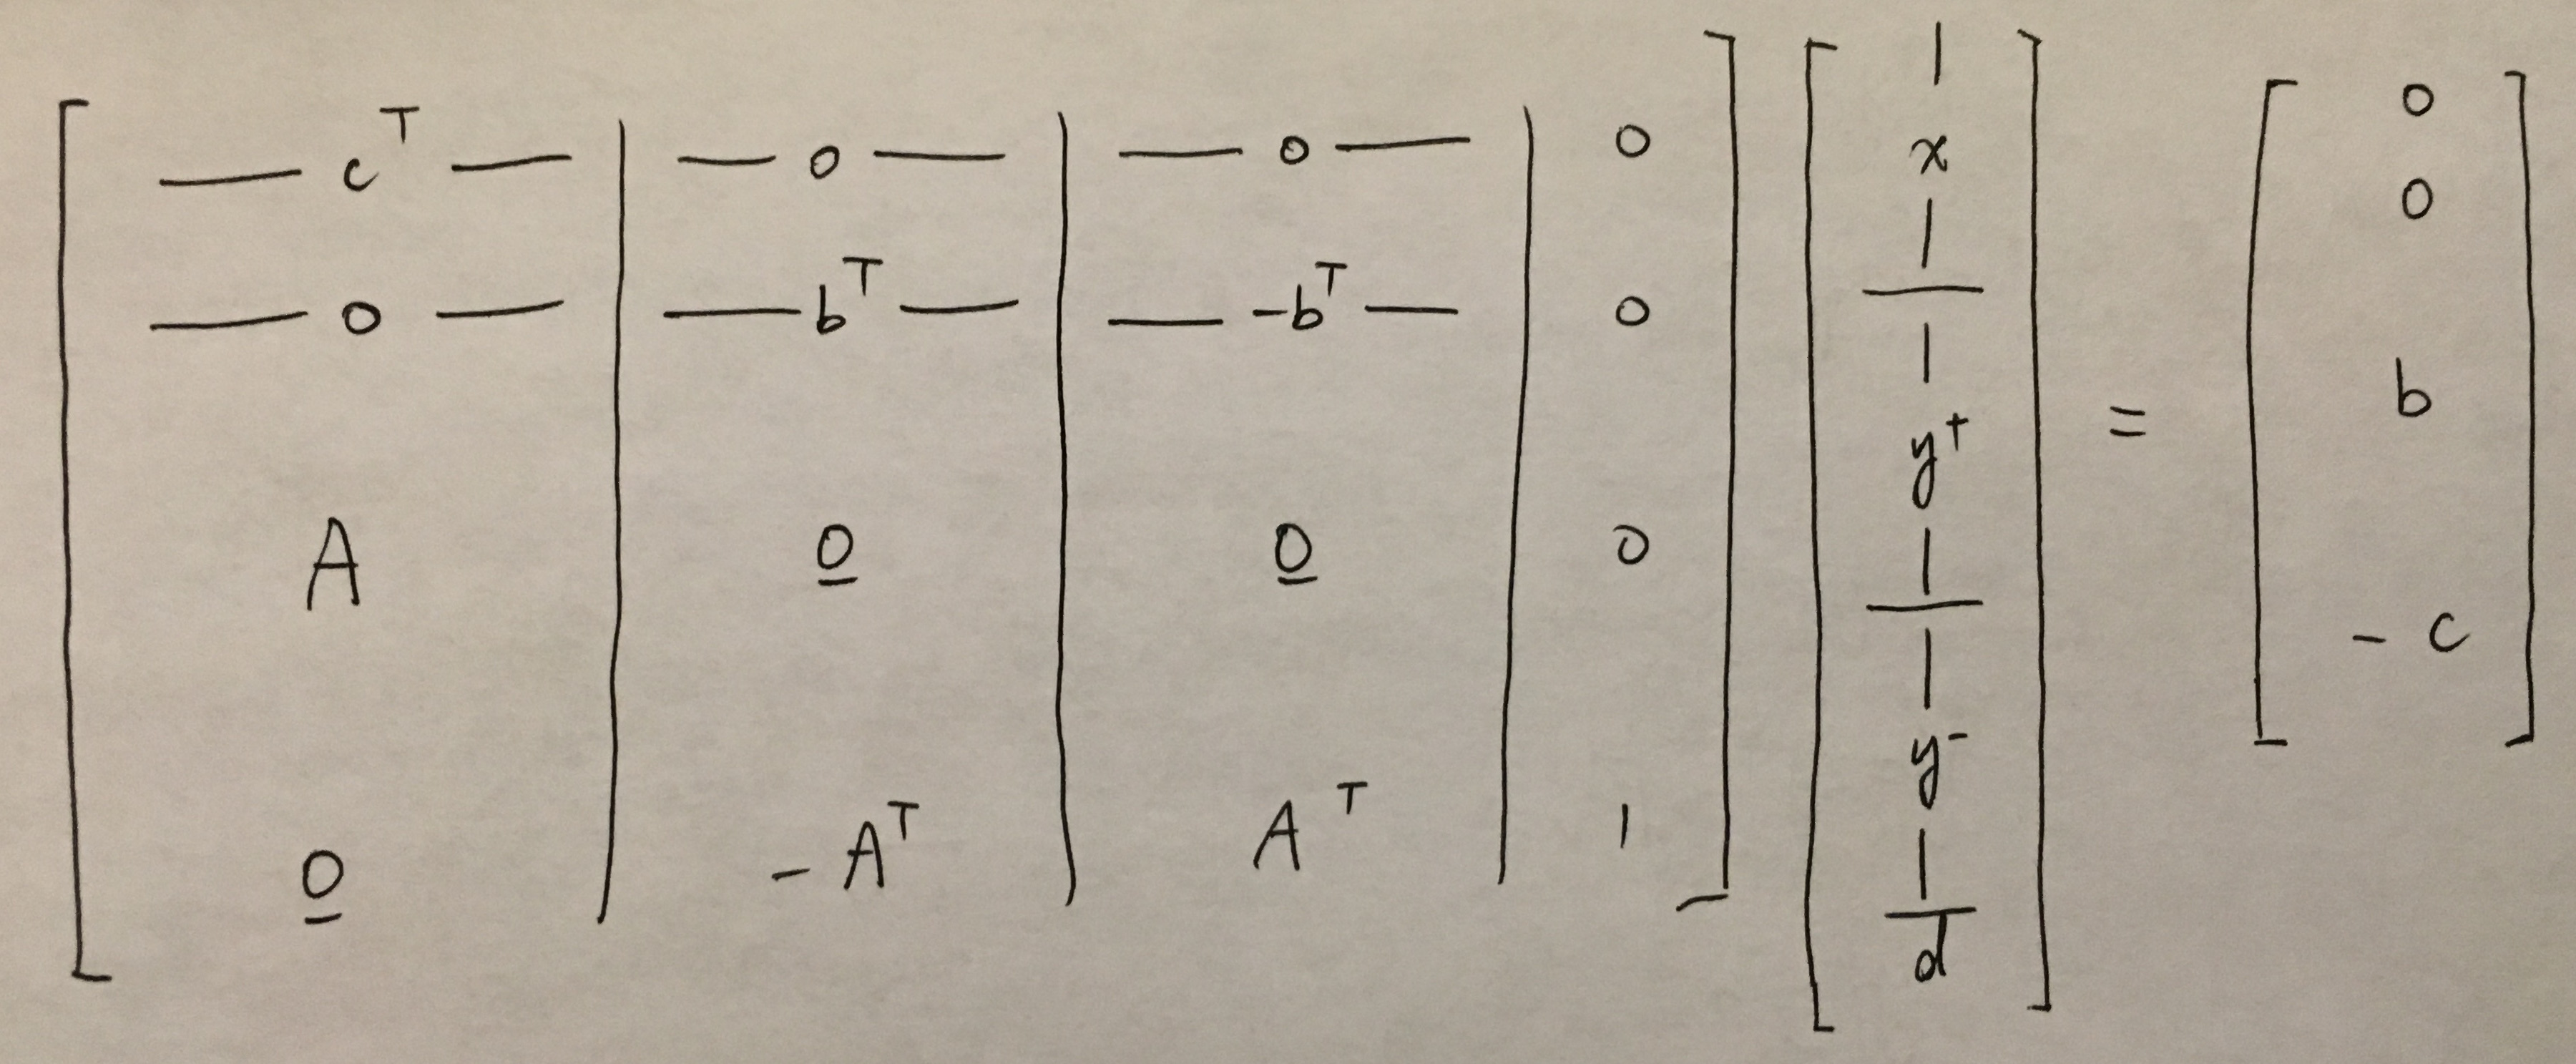
\includegraphics[width=0.7\textwidth]{5-1.jpg}
	\label{fig:5-1}
\end{figure}

\paragraph{(b)}
The dual is 
\begin{align*}
\text{max} ~ b^Ty& \\
\text{s.t.} ~ A^Ty &\leq 0\\
y &~~\text{UIS}.
\end{align*}

\paragraph{(c)}
The solution is 0. This is because when the primal is feasible, dual is feasible and bounded. If $b^Ty$ is less than $0$, then we could have set $y=0$ satisfying the constraint but make the objective $0$ larger than the negative value. If $b^Ty$ is larger than $0$, then we could have \emph{double} the value of $y$, still satisfying the constraints but \emph{double} the objective and make it bigger. 

\paragraph{(d)}
Using (c) we can pass to the algorithm with optimal solution $0$ of dual in (b). Then in $O((m+n)^k)$ time if the algorithm returns and it checks the feasibility in (a), we know the optimal value of original problem is obtained. 

If the return from the algorithm\footnote{the algorithm may not terminate in $O((m+n)^k)$ when the ``solution'' to the dual passed into the algorithm is wrong, in this case we return a random result.} does not pass the feasibility check in (a), it means the original problem is either infeasible or unbounded. 

To check the feasibility, we use the same trick that removes the objective of the original problem and looks into its dual. The dual maximization is $0$ if the primal is feasible. Therefore we invoke the algorithm on the modified original problem with $0$ passed to its dual. If the returned result checks the feasibility test, the original problem is feasible (therefore unbounded because of above), otherwise it is infeasible.

The runtime is asymptotic in $O((m+n)^k)$ because the two calls of the algorithm each has $O(c(m+n)^k) = O((m+n)^k)$ and the checking of feasibility is also in $O((m+n)^k)$.
\end{document}